\section{Theory}
This section explores some of the depth cues that we use to perceive depth. Furthermore, it explores how \textit{stereopsis} and \textit{binocular disparity} is used to construct stereograms.

\subsection{Oculomotor depth cues}
When trying to focus on objects in close range (< 2m) our eye muscles and lenses react by either convergence or accommodation. Convergence means that our eyes turn inward and the lenses take on a rounder shape, when for example trying to focus on objects right in front of the nose. The opposite happens in accomodation, which means that the eyes turn more away from each other until they are almost parallel and the lenses will flatten out again. We sense these muscular reactions and are therefore able to determine depth based on them. However, when objects are further away (> 2m) the reaction become so small that we will most likely not notice them\citep{sensationPerception}.

\subsection{Monocular depth cues}
Monocular depth cues only require a single eye, which means that even though we hold a hand over one eye, we are still able to determine depth based on these cues\citep{sensationPerception}

\subsubsection{Partial Occlusion/interposition}
When object partially hide (or occlude) other objects indicating that the hidden object is behind the non-hidden object(See \autoref{fig:partialOcclusion}). This is called partial occlusion or interposition\citep{sensationPerception}.

\begin{figure}[H]
	\centering
	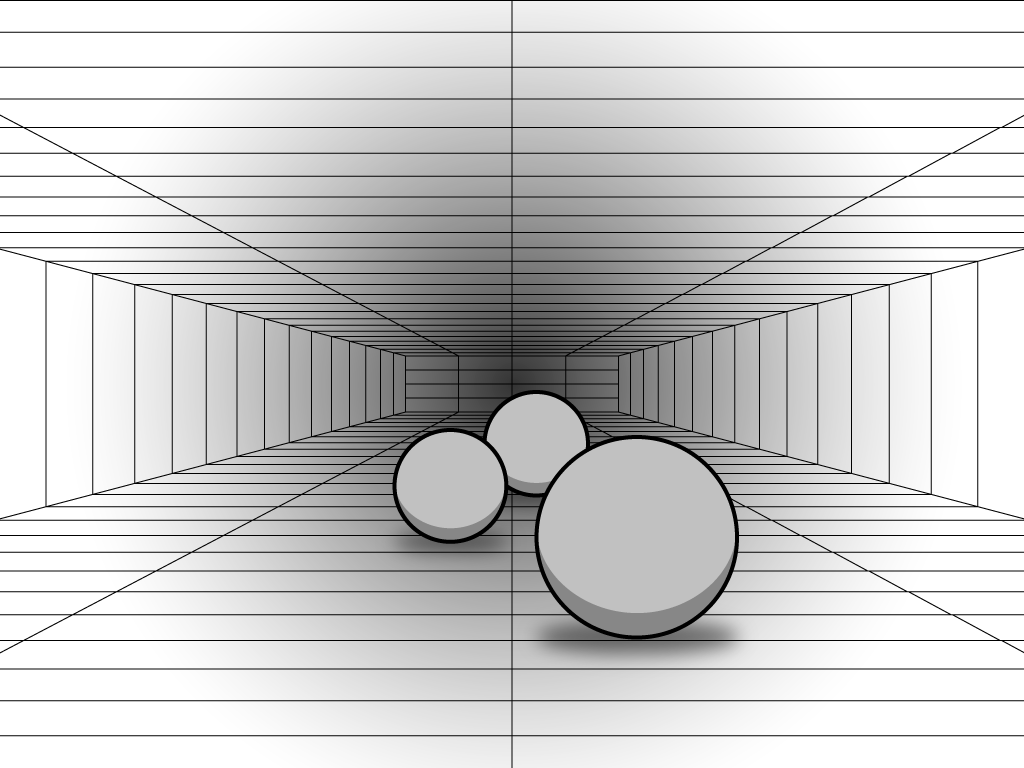
\includegraphics[width=1\linewidth]{figure/Analysis/partialOcclusion.png}
	\caption{Partial occlusion (or Interposition) is a monocular cue that identifies objects which overlap others as closer to the viewer.}
	\label{fig:partialOcclusion}
\end{figure}

\subsubsection{Relative height}
In \autoref{fig:relativeHeight} three round objects can be seen. Although, the three objects to be the exact same size, the position of the objects in the image indicate where they are in 3D space. The object positioned higher up is closest to the horizon in the image and will appear to be further away. In this case the object must also be larger than the object positioned lower in the image. This is called relative height. The opposite would be true for object hanging from the ceiling\citep{sensationPerception}.

\begin{figure}[H]
	\centering
	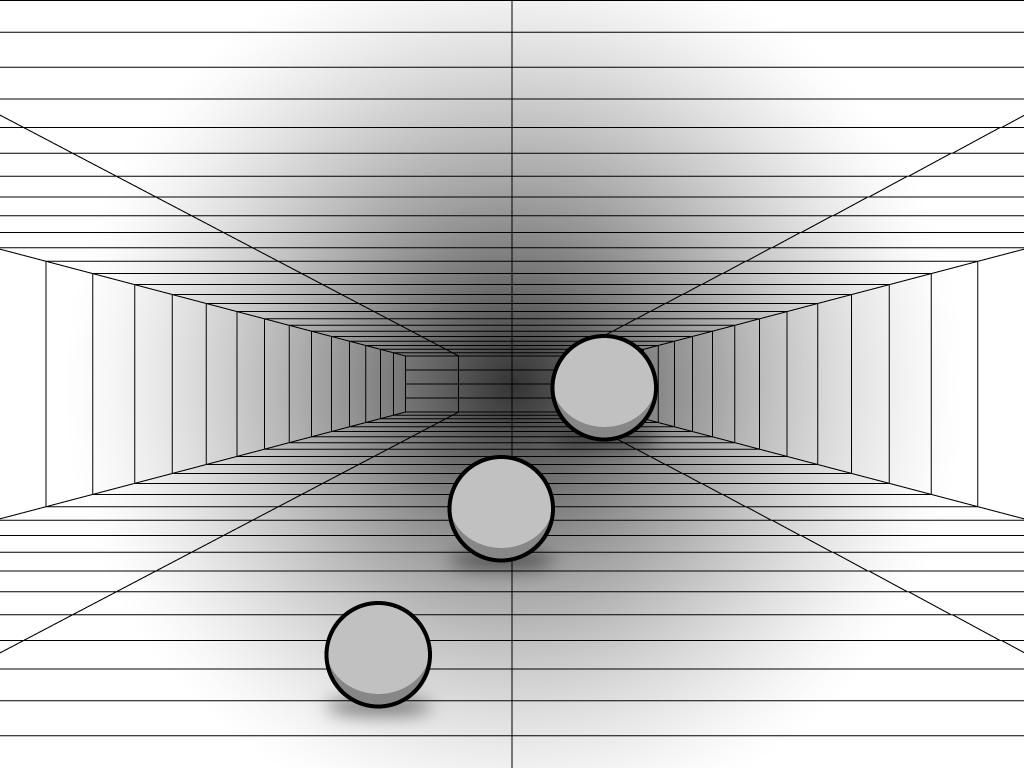
\includegraphics[width=1\linewidth]{figure/Analysis/relativeHeight.png}
	\caption{The position of an object with respect to the horizon in this figure indicate the spatial position of the object.}
	\label{fig:relativeHeight}
\end{figure}

\subsubsection{Relative size}
Assuming that the two objects seen in \autoref{fig:relativeSize} have about the same physical size, we are able to place the objects in space based on how large they appear to be in the image. The larger the object appears, the closer it is\citep{sensationPerception}.
\begin{figure}[H]
	\centering
	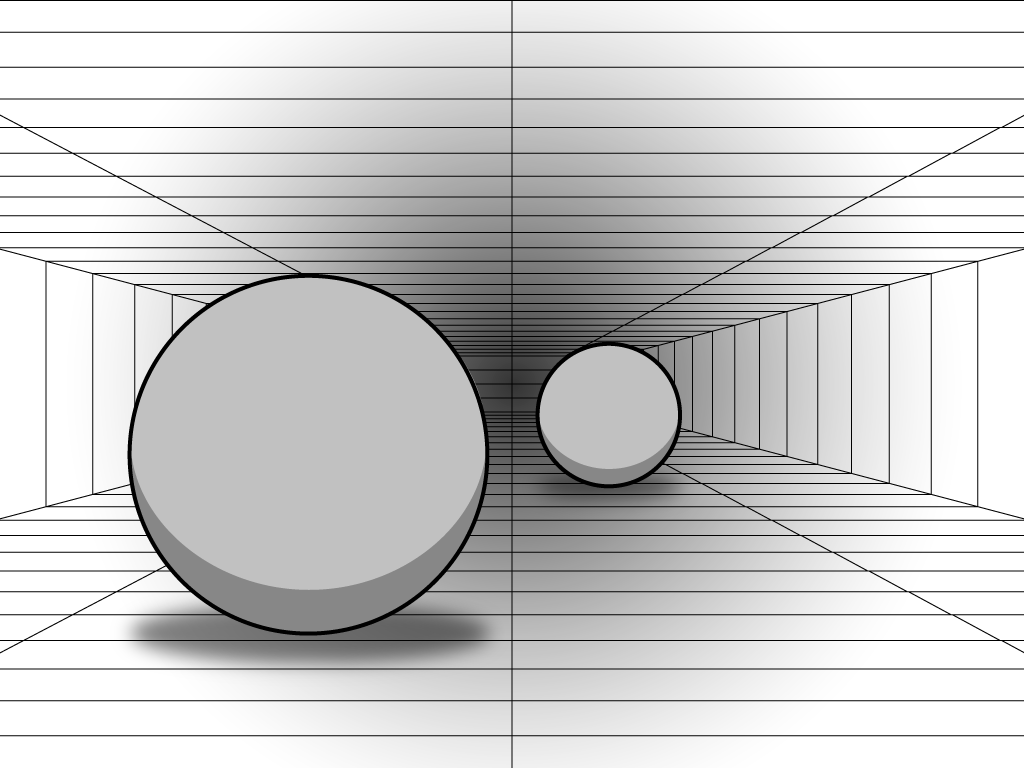
\includegraphics[width=1\linewidth]{figure/Analysis/relativeSize.png}
	\caption{Relative size.}
	\label{fig:relativeSize}
\end{figure}


\begin{figure}[H]
	\centering
	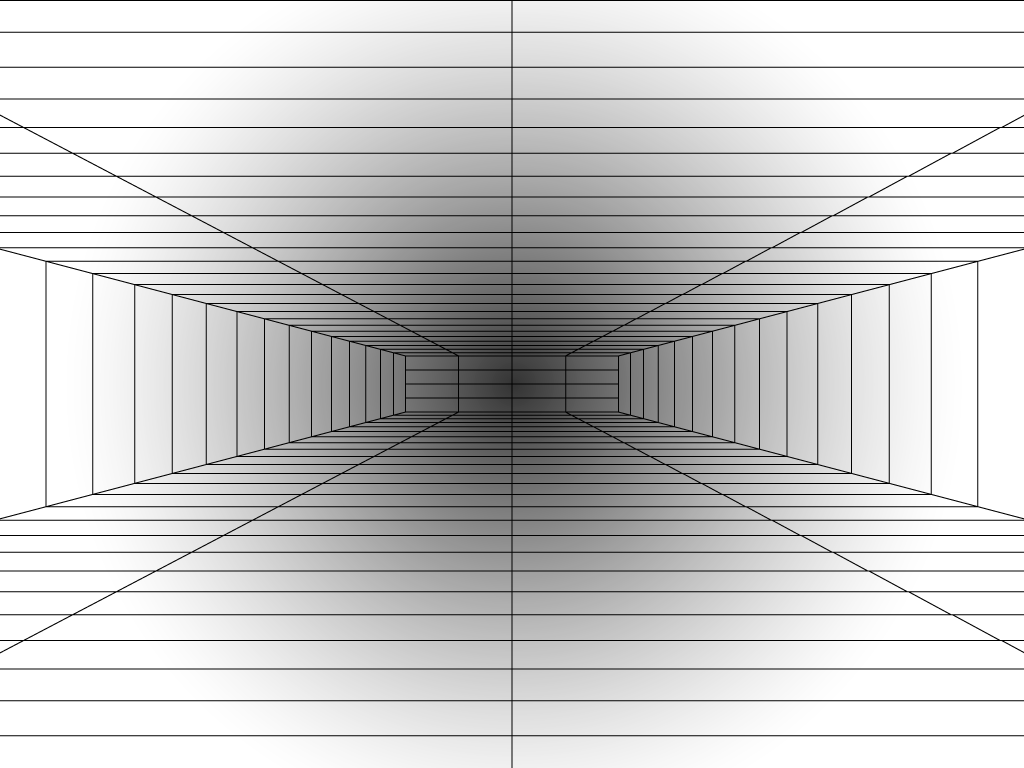
\includegraphics[width=1\linewidth]{figure/Analysis/linearPerspective.png}
	\caption{Linear perspective.}
	\label{fig:linearPerspective}
\end{figure}




\begin{figure}[H]
	\centering
	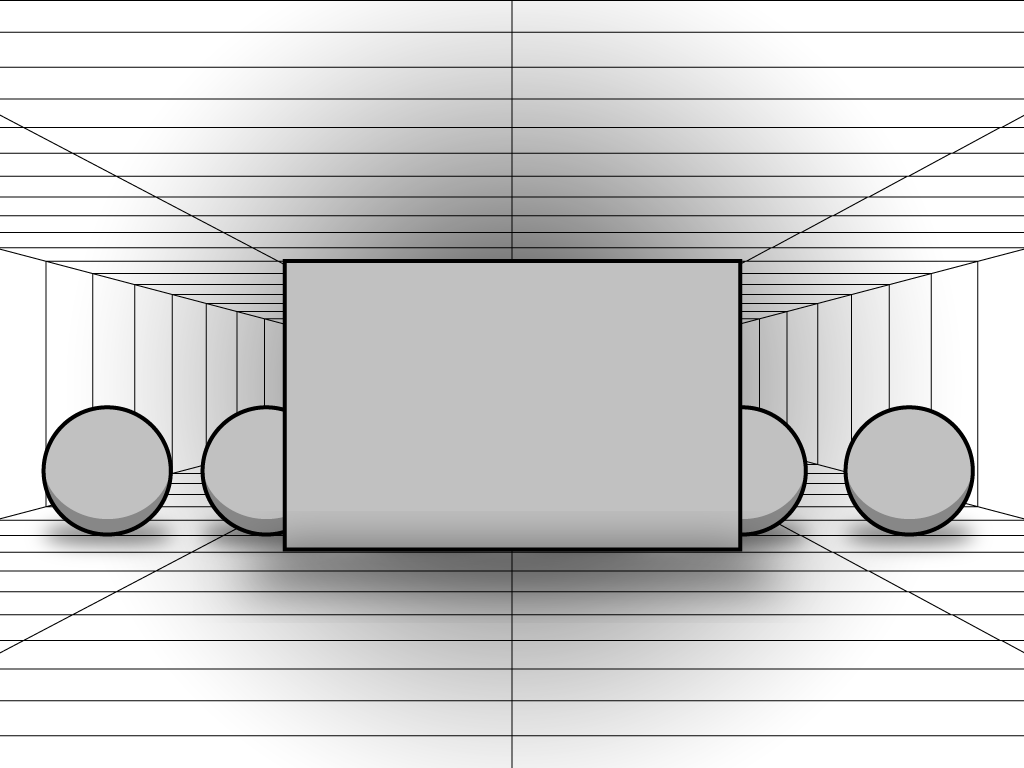
\includegraphics[width=1\linewidth]{figure/Analysis/deletionAccretion.png}
	\caption{Deletion and accretion.}
	\label{fig:deletionAccretion}
\end{figure}

\begin{figure}[H]
	\centering
	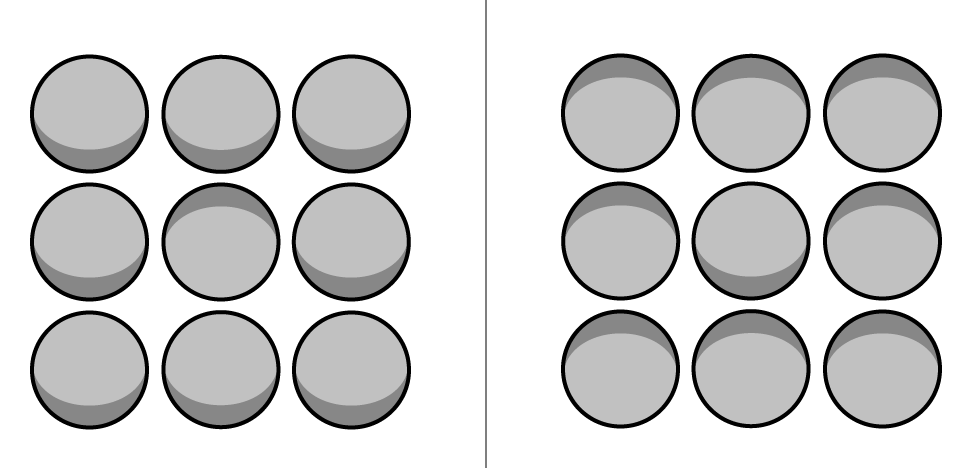
\includegraphics[width=1\linewidth]{figure/Analysis/shading.png}
	\caption{Shading.}
	\label{fig:shading}
\end{figure}

\begin{figure}[H]
	\centering
	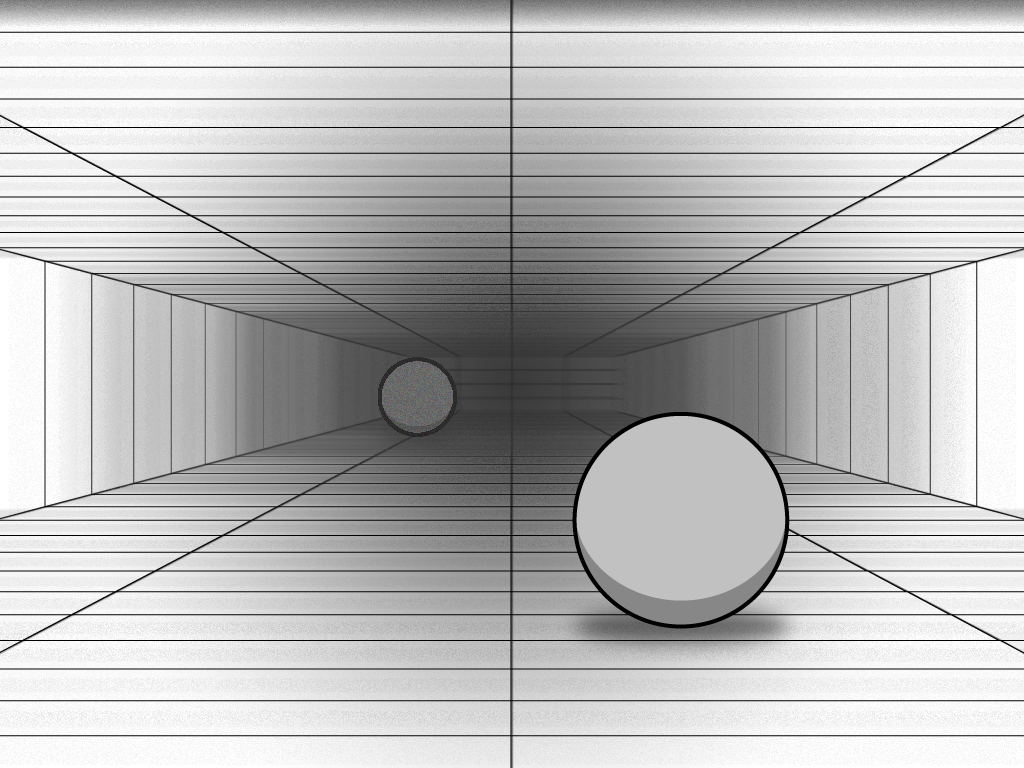
\includegraphics[width=1\linewidth]{figure/Analysis/atmosphericPerspective.png}
	\caption{Atmospheric perspective is a light-based monocular cue. Particles in the air can obscure and distort the retinal information for objects in the distance whereas the objects closest to the viewer appear more clearly.}
	\label{fig:atmosphericPerspective}
\end{figure}


\subsection{Binocular depth cues}
\begin{figure}[H]
	\centering
	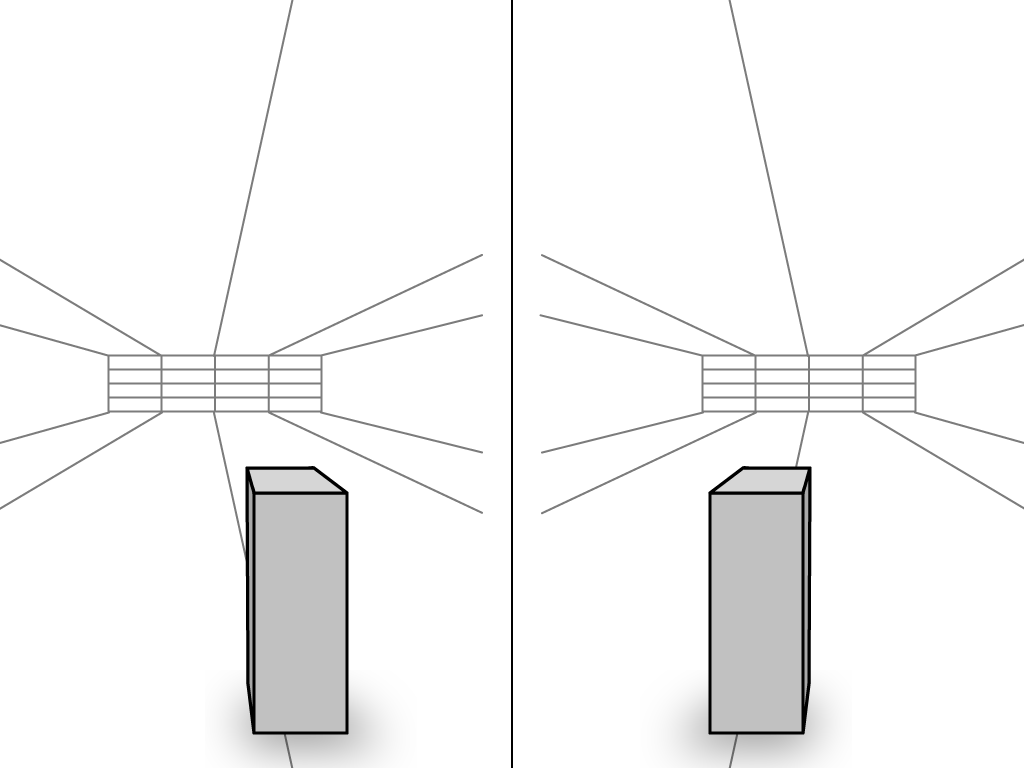
\includegraphics[width=1\linewidth]{figure/Analysis/stereoScopicVision.png}
	\caption{Stereoscopic vision.}
	\label{fig:stereoscopicVision}
\end{figure}


\subsection{Stereopsis and binocular disparity}
Under what conditions do the various cues operate? In particular, explain what is meant by "stereopsis" and "binocular disparity" and how these are used in the construction of stereograms and autostereograms.

\begin{figure}[H]
	\centering
	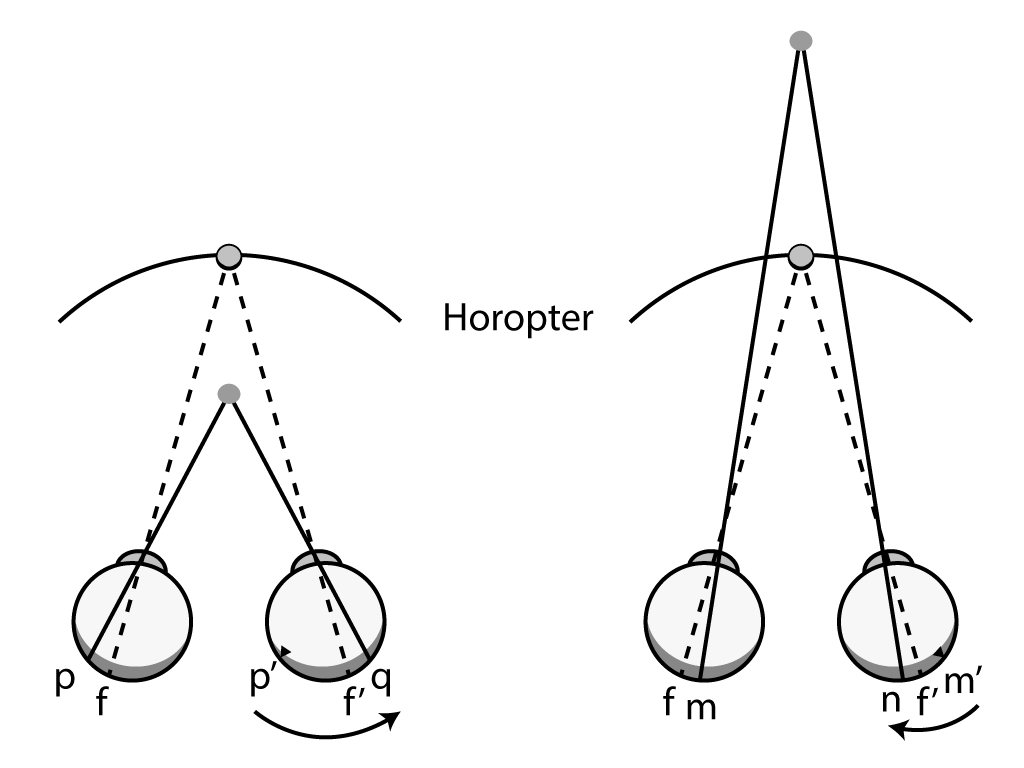
\includegraphics[width=1\linewidth]{figure/Analysis/stereopsis.png}
	\caption{Stereopsis.}
	\label{fig:stereopsis}
\end{figure}


\section{Discussion}

\section{Summary and Conclusion}


